\documentclass[a4paper,11pt]{article}

\usepackage[T1]{fontenc}
\usepackage[utf8x]{inputenc}
\usepackage{fullpage}
\usepackage{amsmath,amssymb}
\usepackage{tikz-uml}
\usepackage{lscape}
\usepackage{pgfplots}
\usepackage{graphicx}
\usepackage{caption}
\graphicspath{{Images}}
\setlength\parindent{0pt}
\setlength\parskip{10pt}

\usepackage[framemethod=tikz]{mdframed}
			\mdfdefinestyle{mpdframe}{
				frametitlebackgroundcolor   =black!15,
				frametitlerule          =true,
					roundcorner     =10pt,
					middlelinewidth     =1pt,
					innermargin     =.20cm,
					outermargin     =0.2cm,
					innerleftmargin     =0.2cm,
					innerrightmargin        =0.2cm,
					innertopmargin      =\topskip,
					innerbottommargin   =\topskip,
						}
			%   Studies
			\mdfdefinestyle{a}{%
					style=mpdframe,
					frametitle={Aside},
				}
			\newmdenv[style=a]{aside}

\title{Bins Are Rubbish}
\author{(JF)$^2$G}
\def\d{\mathrm d}

\begin{document}
	\setcounter{tocdepth}{2}
	\maketitle

	When performing a GCE simulation, it is natural to attempt to simulate the distribution -- and then track the evolution -- of a population of stars born at each timestep $t$. 

	In the assumption of isolated, single stars, the stellar evolution is determined solely by the Zero-Age Main Sequence properties: the Mass, Metallicity and angular momentum. Since angular momentum is (at present) beyond the ability of most stellar evolution models to accurately predict\footnote{Limongi \& Chieffi 2018 tried it. The results were disastrous from a GCE standpoint.}, and the Metallicity is uniquely determined by the time and place of stellar, stellar populations are distributed only in \textit{mass}.

	The most intuitive and obvious means of tracking these populations is therefore by \textit{binning them by mass}.
	
	\section{Why bin?}

		The most obvious answer to the question `why bin by mass in your code?' is `because that was how it was done in the older versions'. But that doesn't give credit to why it's the obvious choice. Consider the following analysis.

		% The old process went something like the following:
		% \begin{enumerate}
		% 	\item At a timestep $p$, form a mass of $M_\text{form}$ of stars.
		% 	\item Split the population into a mass-grid of size $C$
		% 	\item Each bin $i$ has an associated mass $m_i$  (either log-uniform or uniform, it doesn't particularly matter). All stars in the bin are assumed to have mass $m_i$.
		% 	\item Each bin holds $n_{i} = \zeta(m_i)M_\text{form}/\bar{M}$ of the formed stars. 
		% 	\item Each bin has a lifetime $\tau(m_i)$. 
		% 	\item The bin is then predestined to die in a timestep $q = p + \lfloor\frac{\tau(m_i)}{\Delta t}\rfloor$
		% 	\item At timestep $q$, inject matter yields equal to $n_i m_i Y(m_i,Z)$ back into the galaxy
		% \end{enumerate}

		During the $j^\text{th}$ timestep, a mass $M_\text{form}$ of stars forms out of gas. We assume (for the sake of generality) that the IMF can be dependent on the metallicity:
		\begin{equation}
			\zeta = \zeta(M|Z)
		\end{equation}
		The average mass of a star formed at metallicity $Z$ is
		\begin{equation}
			\bar{M}(Z) = \int_0^\infty M \zeta(M|Z) \mathrm d M
		\end{equation}
		Both the total number of stars ($N$) formed from a mass $M_\text{form}$, and the distribution of each mass ($n$) are simple:
		\begin{equation}
			N_\text{form}(Z) = \frac{M_\text{form}}{\bar{M}(Z)} ~~~ \Longleftrightarrow~~~n_\text{form}(M,Z) = \zeta(M|Z) N_\text{form}(Z)
		\end{equation}

		We then compute:
		\begin{equation}
			n_i = N_\text{form}(Z) \int_{M_-(i)}^{M_+(i)}\zeta(M|Z) \d M ~~~~~~~ m_i = \int_{M_-(i)}^{M_+(i)}\zeta(M|Z) M \d M 
		\end{equation}
		% When it came time to compute the value of some arbitrary function $f(M)$ evaluated across the entire population, we would then find:
		% \begin{equation}
		% 	F[f] \approx \sum_{i=0}^C f(m_i) n_i
		% \end{equation}

		% For example, the total mass of the stellar population could be found by setting $f(M) = M$, in which case the sum counts the masses of all surviving stars. 
		As time progresses, stars in this population will die off, and so $n_i$ must be modified. This can easily be achieved by also computing the timestep during which the stars will die. With $\delta$ equal to the simulation timestep:
		\begin{equation}
			t_i^\text{death} = t^\text{born} + \left\lfloor\frac{\tau(m_i)}{\delta} \right\rfloor
		\end{equation}
		At this timestep, we set $n_i = 0$, and those stars exit the population. Quantities which arise from those deaths can be computed (before $n_i$ is set to zero) by the sum:
		\begin{equation}
			F[f_\text{death}](t_\text{now}) = \sum_{i \in \{t_i^\text{death} = t_\text{now}\}} f_{\text{death}}(m_i) n_i \label{E:DeathBins}
		\end{equation} 
		For example, the total mass of stars dying (and hence the ejecta mass returned to the ISM - modulo finite-mass remnants) can be recovered by setting $f_\text{death}(M) = M$, the AGB rate by a function which is 1 below $M_\text{CCSN}$ and 0 above, and similarly with the yields, and so on.

		The mass-binning occurred because it seemed like the most obvious way to compute the time period at which each star would die, and thus what material would be returned back to the ISM at that time. The thinking was, simply, that if the mass bins were small enough, then the properties would be approximately constant across the bins. 

		

		The problem, however, is that whilst this holds true for the yield properties, it is resolutely not true for the isochrone-derived properties, which have A Lot Going On in the [0.5,2] $M_\odot$ range - most notably ranging in lifetime from $>50Gyr$ down to $<3Gyr$. Given that our mass bins must extend up to $100M_\odot$, the required resolutions to truly capture the behaviour in this tiny region is immense.

	\section{A World Without Bins}
		It is our assertion that it is entirely possible to compute the relevant properties for a GCE simulation without requiring a mass-gridded population. 
		
		\subsection{The Integrals}

			The key quantity we will be working with is a reformulation of $F[f]$ in Eq.\eqref{E:DeathBins}, but one which is not limited merely to computing death-time quantities. We could compute arbitrary population-aggregate quantities by:
			\begin{equation}
				F[f](t) \approx \sum_i f(m_i,t) n_i
			\end{equation}
			We recover by Eq.\eqref{E:DeathBins} in the case where $f(m_i) = 0$ whenever $t \neq t^\text{death}_i$. We realise that this formulation is itself a discretised form of the integral\footnote{We could also formally prove this in the limit that the mass-bins become infinitely small, $C\to\infty$, $\delta m \to 0$.}
			\begin{align}
				\begin{split}
				F[f](t,Z) & = \int_0^\infty n_i(M,Z) f(M,Z,t) \d M
				\\
				& = N_\text{form} \int_0^\infty \zeta(M|Z) f(M,Z,t) \d M
				\\
				& = N_\text{form}  \mathcal{R}[f](Z,t)
				\end{split}\label{E:FormalStatement}
			\end{align}
			These $\mathcal{R}[f]$ depend only on the simulation timestep ($t$) and the metallicity $Z$. We know the timesteps in advance, and we are relatively happy with simple linear interpolation of metallicity\footnote{Metallicity dependence is important, but rarely has a strong gradient.}. We can therefore precompute them across the known simulation times and a proscribed $Z$-grid, when the time comes to query a stellar population it is then a trivial matter to compute $\mathcal{R}[f](Z,t)$, and hence $F[f](t)$, for an arbitrary stellar population. 

			This is a roundabout way of expressing something perhaps obvious, given we explicitly limit ourselves to the continuum limit: the behaviour (fraction dying at a certain time, etc.) of a population of stars is independent of the number of stars in the population.

			% Rather than attempting to rifle through the currently-living members of a population to determine which stars have reached the end of their lifetime (and which meet certain conditions) - so long as those conditions are predetermined, then we can replicate this by multiplying the initial population mass by some matrix value, and then interpolating over $Z$.

		\subsection{The Finite-Resolution Death Distribution}
			With the exception of simulating the final stellar population (which we ignore for now), all values we are interested in computing occur at the end of a star's lifetime. We must reliably be able to compute which stars are dying in a given time bin. 

			We assume that we possess an analytic function $\tau(M)$ which gives the lifetime of a star of mass $M$, and its inverse $M(\tau)$. This assumption is relaxed in \S\ref{S:Interpolation}.

			The most natural assumption is that $f$ acts to truncate the integral \eqref{E:FormalStatement} to $[M(t),M(t+\delta)]$, where $\delta$ is the width of a timestep. That is to say, we integrate only over masses which have lifetimes which fall within the current timestep.
			\begin{equation}
				\mathcal{R}[f](Z,t) = \left|\int_{M(t)}^{M(t+\delta)} \zeta(M|Z) f(M,Z,t) \d M \right|
			\end{equation}
			The $|x|$ was introduced so that we didn't have to worry about the sign of $\frac{\d M}{\d t}$, and hence about the ordering of $M(t)$ vs $M(t+\delta)$. 
			
			However, this formulation assumes that 100\% of stars with lifetimes in the range $[t,t+\delta]$ die during this time bin. However, since time bins represent a \textit{range} of times, it is also possible for their \textit{births} to be distributed across the time bin. A star with lifetime $t+\delta$ will only die in the $[t,t+\delta]$ bin if it was born precisely at $t = 0$. If it was born at $t = \delta/2$ (i.e. halfway through the first timestep), it will actually die in the \textit{next} timestep.

			\def\W{\mathcal{W}}
			To allow such `overspill', we introduce the Finite-Resolution Death-Distribution. This function determines the probability that a star born during the $i^\text{th}$ window with lifetime $\tau$ dies during the $j^\text{th}$ window.

			If $t_i$ is the $i^\text{th}$ temporal bin (with associated width $\delta_i$) and similarly for $t_j, \delta_j$, then the fraction of stars born at time $t_i \leq t < t_i + \delta_i$ with lifetime $\tau$ which die during $t_j \leq t < t_j + \delta_j$ is a trapezoid distribution:

			\begin{align}
				\W(\tau|i,j) & = \begin{cases} 0 & \tau \leq T_-
					\\
					\frac{\tau - T_-}{\delta_i} ~~~~& T_- < \tau \leq R_1
					\\
					\text{min}\left(\frac{\delta_j}{\delta_i}, 1\right) & R_1 < \tau \leq R_2
					\\
					\frac{T_+ - \tau}{\delta_i} & R_2 < \tau \leq T_+
					\\
					0 & \tau > T_+
				\end{cases}
				\\
				T_- & =  t_j - t_i - \delta_i
				\\
				R_1 & = T_- + \text{min}(\delta_i, \delta_j)
				\\
				R_2 & = R_1 + |\delta_i - \delta_j|
				\\
				T_+ & = t_j - t_i + \delta_j
			\end{align}


				In the case that $\delta_i = \delta_j = \delta$, a uniform temporal resolution, this reduces to a simple triangular distribution:

				\begin{align}
					\W(\tau|t) & = \begin{cases} 0 & \tau \leq T_-
						\\
						\frac{\tau - T_-}{\delta} ~~~~& T_- < \tau \leq t
						\\
						\frac{T_+ - \tau}{\delta} &  t < \tau \leq T_+
						\\
						0 & \tau > T_+
					\end{cases}
					\\
					T_\pm & =  t \pm \delta
				\end{align}

			% \subsubsection{The Resulting Integral}

				The result of this is a modified form of $\mathcal{R}$ which allows for stars to blur over the edges of time bins:
				\begin{equation}
					\mathcal{R}^\text{lifetime}[f](Z,t) = \left|\int_{M(t-\delta)}^{M(t+\delta)} \zeta(M|Z) f(M,Z,t) \W\left(\tau(M,Z),t\right)\right|
				\end{equation}

			\subsubsection{Non-Mononicity}
				I have implicitly assumed in the above that $\tau(M)$ is monotonic, and hence that $M(\tau)$ is a unique inverse. This is not guaranteed to be the case (lifetime inversions can be seen around $M\sim 1.7M_\odot$).

				This does not alter the above formulations - instead we simply have to sum over all subregions where $T_- < \tau(M) < T_+$.

		\subsection{A Demonstration}


			To demonstrate the issues inherent with mass-binning, and how this is solved with our $\mathcal{R}$-based approach, we build a toy model of a GCE simulation. We make the usual assumptions of a single gas reservoir, well mixed, continuum limit, and so on. 

			The reservoir begins with an initial gas mass $M_0 = 5\times10^9 M_\odot$, and new gas is added to the reservoir at a rate:
			\begin{equation}
				\dot{M}_\text{gas}^\text{onfall}(t) = \left[5\exp\left(-\frac{t}{3}\right) + 10(t-1)\exp(-(t-1)) \Theta(t-1)\right]\times 10^9 M_\odot \text{Gyr}^{-1}
			\end{equation}
			Where $t$ is measured in Gyr, and $\Theta$ is the usual step function. Stars form from this gas mass according to the usual K-S formation law:
			\begin{equation}
				\dot{M}_*^\text{born} = 0.5 M_\text{gas}^{1.3}
			\end{equation}
			Stars are born with masses distributed according to a simple Miller-Scalo IMF:
			\begin{equation}
				\zeta(M) = \begin{cases}
				\frac{\alpha - 1}{\alpha} & 0 < M\leq 1
				\\
				\frac{\alpha - 1}{\alpha} M^{-\alpha} & M > 1
				\end{cases}
			\end{equation}
			We use the standard $\alpha = 2.3$.

			We use an entirely artificial stellar lifetime model, which is tuned merely to give approximate order-of-magnitude correctness. We choose:
			\begin{equation}
				\tau(M) = \begin{cases} \tau_c \exp\left(-\beta(M- M_c)\right) & M < M_c
					\\
					~
					\\
					\frac{\tau_c}{\gamma(M-M_c) + 1} & M\geq M_c
				\end{cases}
			\end{equation}
			Where
			\begin{equation}
				\tau_c = \tau_\odot \exp\left(-\beta(M_c- M_\odot)\right)
			\end{equation}
			This function is monotonically decreasing, tuned to give $\tau(M_\odot) = \tau_\odot$, and is continuous around the critical point $M_c$, but has discontinuous gradient, unless $\beta = \gamma$. We explore how varying these values impacts the model. The inverse of this function can be found to be:
			\begin{equation}
				M(\tau) = \begin{cases}
					M_c - \frac{1}{\beta} \log\left(\frac{\tau}{\tau_c}\right) & \tau > \tau_c
					\\
					M_c + \frac{1}{\gamma} \left(\frac{\tau_c}{\tau} - 1\right) & \tau \leq \tau_c
				\end{cases}
			\end{equation}

			\begin{figure}
				\begin{center}
				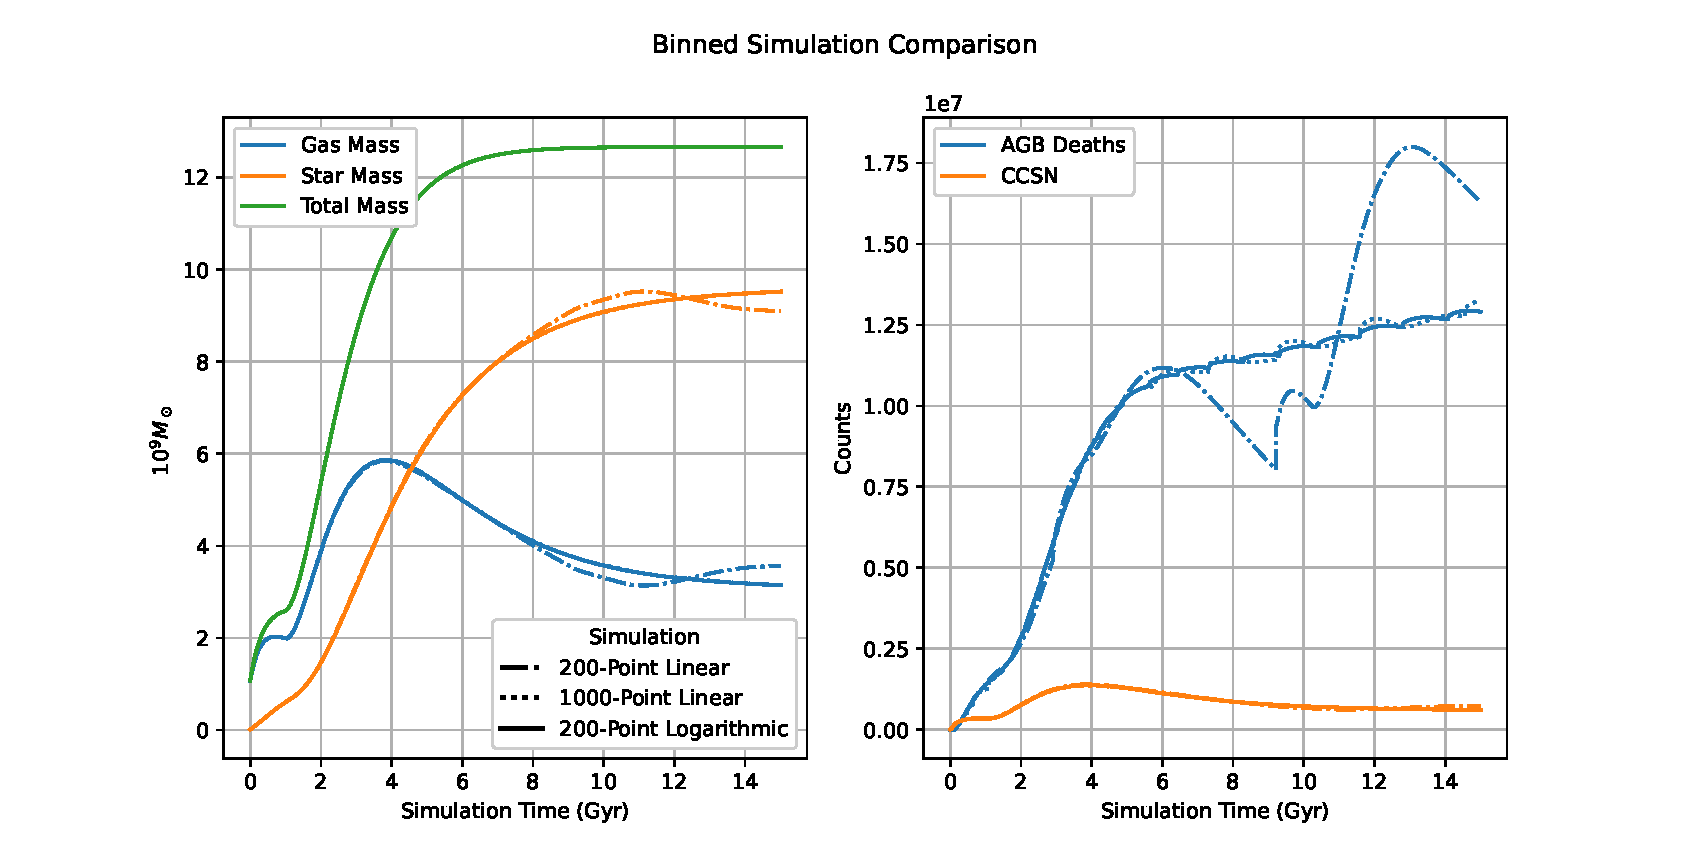
\includegraphics[width=\linewidth,height=0.4\paperheight,keepaspectratio=true]{BinnedSim_Pulsing.eps}
				\caption{The basic toy model with a $\beta = \gamma = 2.3$. The different line-styles denote different resolutions of the mass bin. Linear bins are uniformly space with $m_i - m_{i-1} = \delta m$, logarithmic bins have $\log(m_i) - \log(m_{i-1}) = \delta m$}\label{F:PulsingModel}
				\end{center}
			\end{figure}

			\subsubsection{Simulations \& Comments}

				Figure \ref{F:PulsingModel} demonstrates the basic toy model with varying resolutions of the mass bins. We see that at ``low'' linear-resolutions ($C = 200$, so $\delta m = 0.5 M_\odot$) the AGB rate varies wildly across time, which is not seen at higher resolutions, or when the mass grid is logarithmic: the properties of stars vary on much smaller scales than $0.5 M_\odot$ at small masses, and this has galactic-scale impacts, as we can see the linear model has deviating galactic gas and star balances compared to the higher resolutions: the choice of mass binning can drastically alter the mass balance of the galaxy.

				Even at high resolutions, however, we see that the galactic AGB death-rate `pulses', with time. This results in discontinuous amounts of gas being returned to the galaxy, which would drive a `bursty' star formation rate, and also discontinuous enrichment profiles.


				\begin{figure}
					\begin{center}
					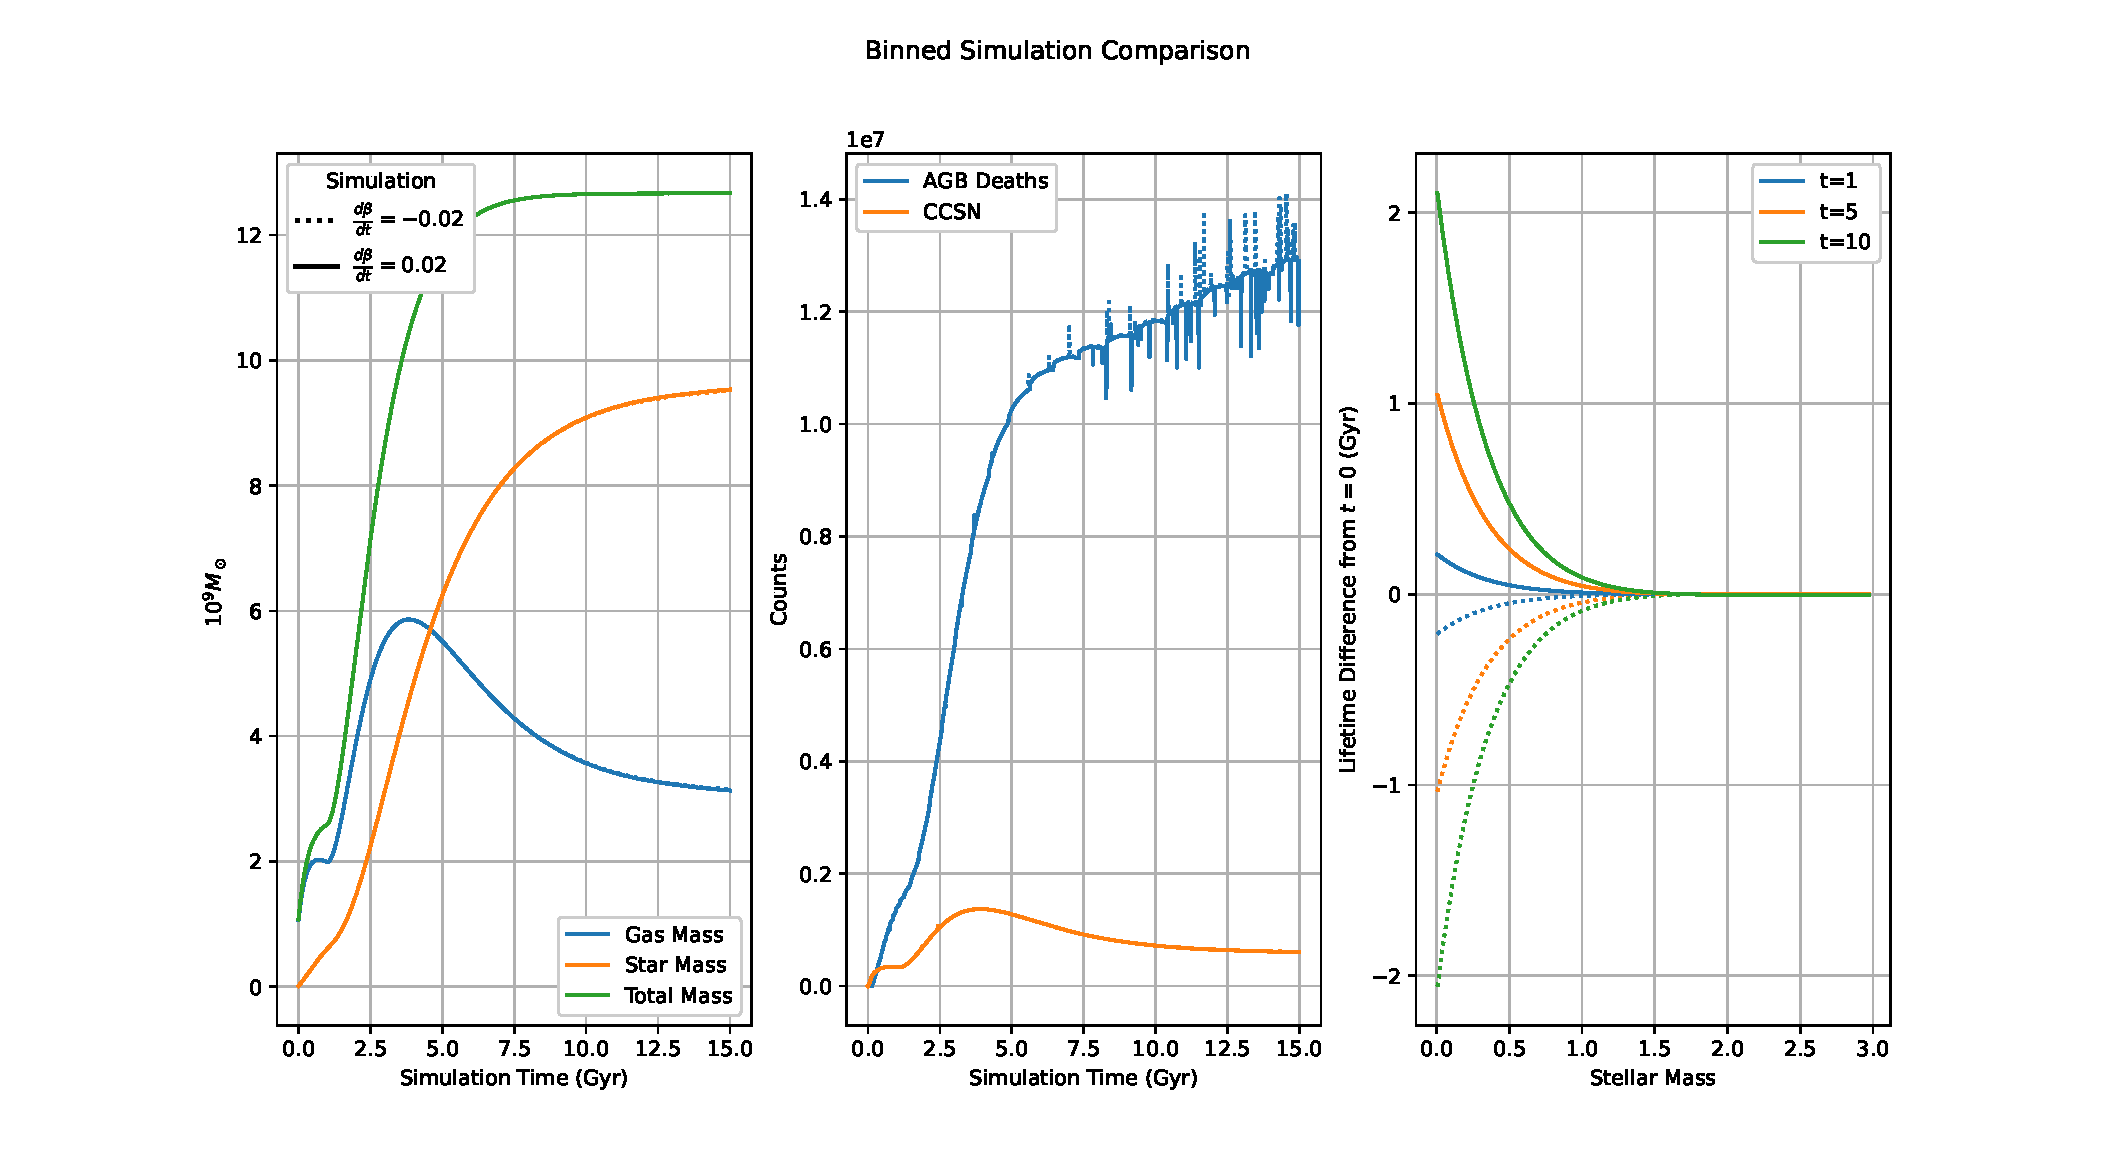
\includegraphics[width=\linewidth,height=0.4\paperheight,keepaspectratio=true]{BinnedSim_Spiking.eps}
					\caption{As with Fig. \ref{F:PulsingModel}, but the mass bins are constant (logarithmic, $C = 200$). Instead we allow the exponent of the lifetime function to vary with time, mimicking a metallicity dependence on lifetime. The right hand panel shows the change in lifetime from the $\beta = 2.3$ model for stars of different masses, born at different times.}\label{F:SpikingModel}
					\end{center}
				\end{figure}

				The situation is made even more disconcerting when one allows for the possibility that $\tau = \tau(M,Z)$ - that is, the lifetime of populations can vary as the reservoir evolves. We know that metallicity is a driver of variability in stellar lifetimes, but rather than attempt to simulate a full metallicity/lifetime relationship in our toy model, we choose to make $\beta$, the exponent for low mass stars\footnote{and since $\gamma = \beta$, the prefactor for high-mass stars}, vary with time. We choose the form:
				\begin{equation}
					\beta(t) = 2.3 + \nu \times t
				\end{equation} 

				Fig. \ref{F:SpikingModel} shows the result of $\nu = \pm 0.02$. From the right hand panel, we see that even though the variation in lifetime for stars which actually perish is $<0.1$Gyr, the result on the AGB rate is striking: no longer do we have simple `pulses', but instead sharp, discontinuous spikes, the result of stars `bunching up' within timestep bins in a way that is not nicely cancelled by stellar populations with the same pattern of `bunching' in their mass bins: since each stellar population now `bunches' differently depending on their stellar lifetimes they were assigned. 

				We have observed this behaviour in both RAMICES I and RAMICES II. This model demonstrates that it is an inherent property of models which a) have mass bins and b) have stellar lifetimes which are not simply $\tau = \tau(M)$.



				\begin{figure}
					\begin{center}
					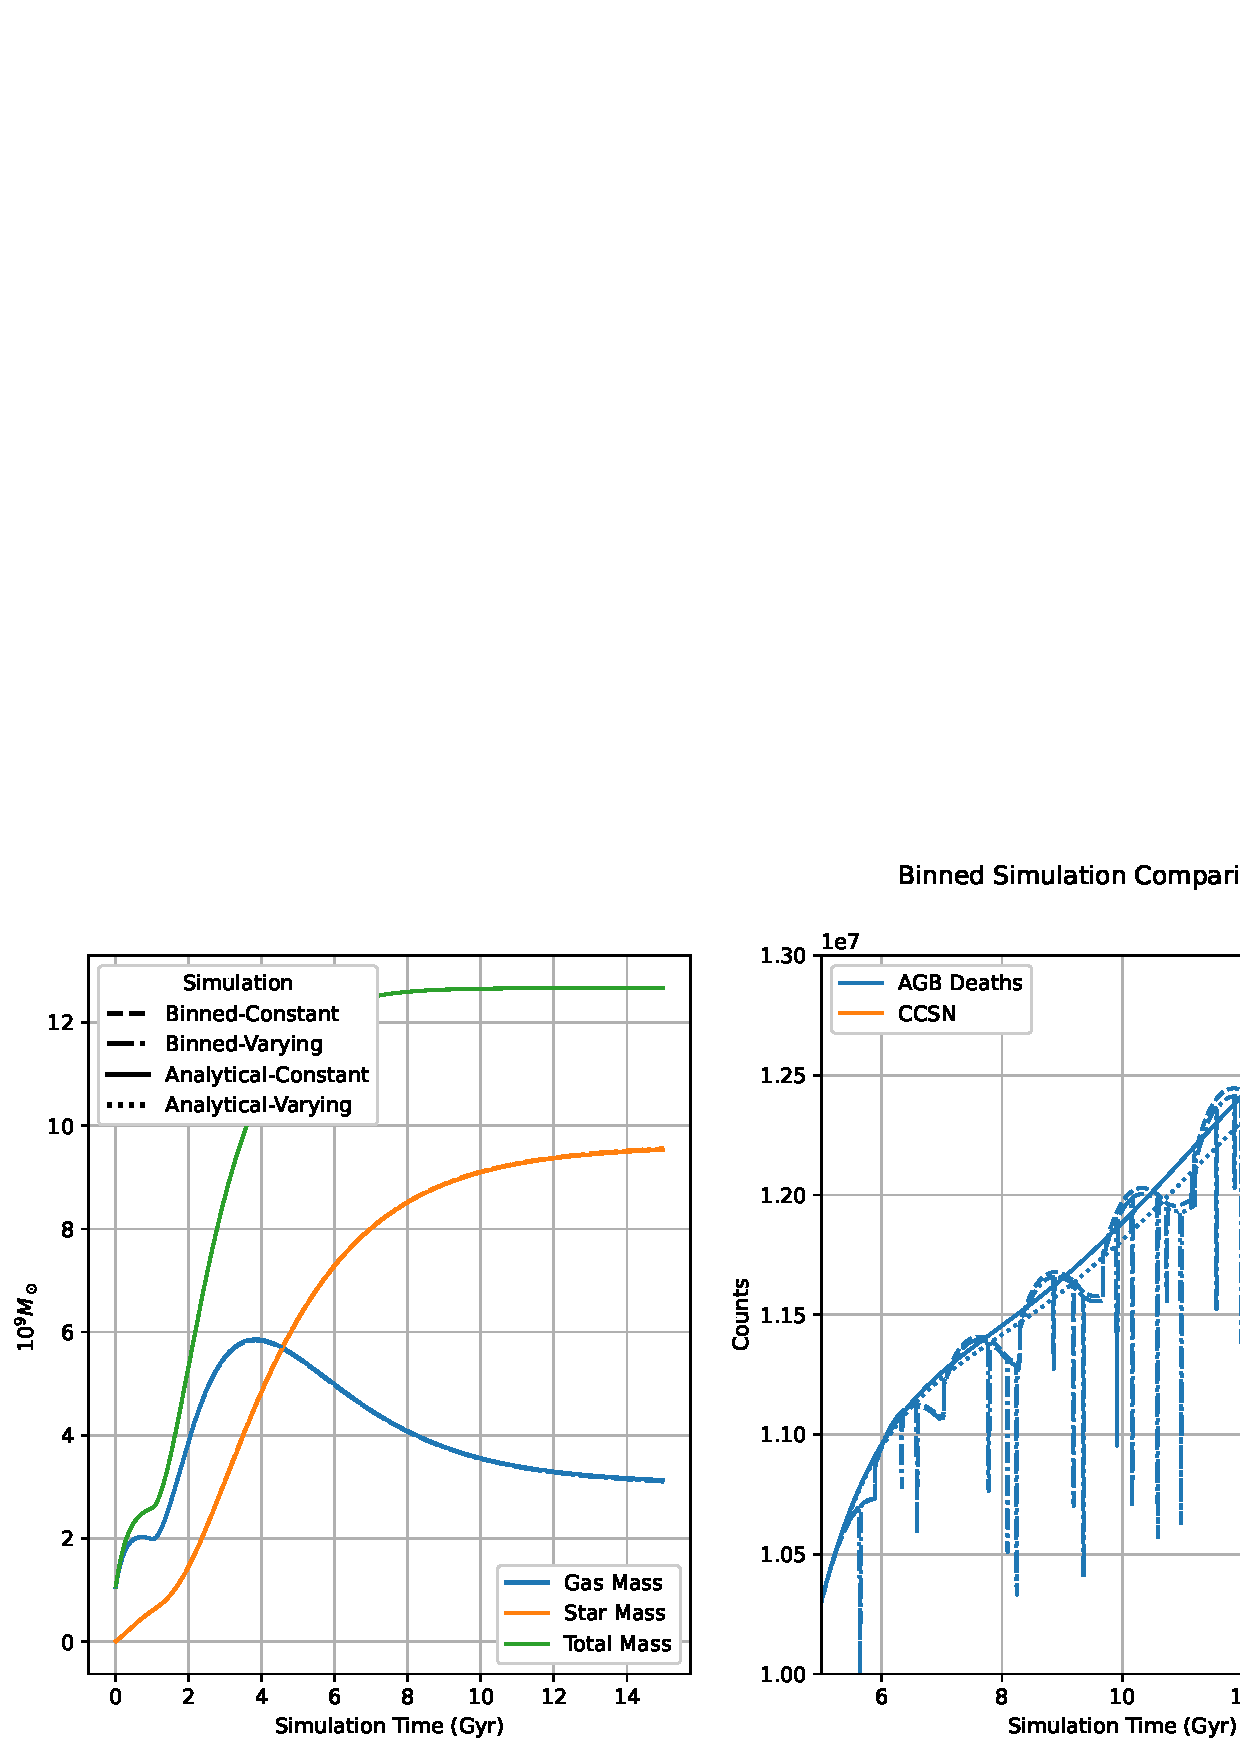
\includegraphics[width=\linewidth,height=0.4\paperheight,keepaspectratio=true]{BinComparison_Varying.pdf}
					\caption{As with Fig. \ref{F:SpikingModel}, with the addition of non-mass binned models (`analytical'). `Varying' models have $\frac{\d\beta}{\d t} = 0.04$, whilst in `Constant' models this is zero. The centre panel shows the global AGB rate zoomed in to demonstrate the differing behaviour, with the Binned-Analytic model plotted with low transparency for ease of interpretation. In contrast, the right panel shows the fractional AGB and CCSN rate \textit{from a single population of stars}. This is evaluated at $t = 10$ for the time-varying models. }\label{F:AnalyticModel}
					\end{center}
				\end{figure}

				In contrast, in Fig. \ref{F:AnalyticModel} we demonstrate the power of the analytical formulation developed above. For these models we computed the mass-return matrix $\mathcal{D} = \mathcal{R}[M]$, the AGB-rate matrix $\mathcal{A} = \mathcal{R}[\Theta(M_\text{ccsn} - M)]$ and CCSN-rate matrix $\mathcal{C} = \mathcal{R}[\Theta(M - M_\text{ccsn})]$. In the case where we had `metallicity dependence' (we reiterate that we spoof this with a time dependence), we evaluated them on a 15-point grid and interpolated linearly between them\footnote{We also tried this with a 100-point interpolation. The difference between them was too small to observe, so we concluded that a resolution of 15 was sufficient.}. 

		\subsection{Conclusions}

			We have demonstrated in this section that mass binning in GCE simulations inherently brings with it myriad problems. These are magnified when the lifetime of stars is not a constant function, resulting in unphysical spikes in the global AGB rate.

			However, we have demonstrated that these spikes can be robustly dealt with and identified by means of a precomputable, integral-based approach. These integrals require a small amount of overhead to compute, but once computed run significantly faster than the binned simulations (since a binned algorithm has a runtime linear in the number of bins). We saw a speedup in excess of $10\times$ at the highest bin-resolution, and 3$\times$ at a moderate resolution. There is also the consideration of a considerable memory saving, since each stellar population no longer needs a vector of mass bins.  

			We note additionally that the additional overhead is marginal, requiring only a few seconds to compute to a high degree of accuracy in Python. When ported to the full C++ simulation, the overhead should be negligible. 
	\section{Gridded Lifetimes}\label{S:Interpolation}
	
		In the prior section, we assumed that both $\tau(M,Z)$ and $M(\tau,Z)$ were provided to us as functional forms, such that we could compute them to arbitrary accuracy. 

		This is not generally the case. Instead, we derive these functions from isochrone data, which is tabulated in $(M,Z)$. We must therefore generalise some means of deriving what the value of $\tau$ might be in between two datapoints. 

		We might naturally assume that a linear interpolation scheme is the most natural, that is, if $M_i < M < M_{i+1}$, then:
		\begin{equation}
			\tau(M) \approx \tau_i + \frac{M - M_i}{M_{i+1} - M_i} \left(\tau_{i+1} - \tau_i\right)
		\end{equation}
		Alternatively, if we expect the relationship to be a powerlaw, then an interpolation in logarithmic space might be better:
		\begin{equation}
			\log(\tau(M)) \approx \log(\tau_i) + \frac{\log(M/M_i)}{\log(M_{i+1}/M_i)} \log\left(\tau_{i+1}/\tau_i\right)
		\end{equation}
		The interpolation scheme is not something we can simply take for granted, since we know that in the region $[0.5,3]M_\odot$ lifetimes vary between $[1,50]$Gyr -- and we want simulation resolutions of order $\delta \approx 10^{-2}$Gyr. This means that unless we have an extraordinary number of isochrones in our tabulated data, there will be many points for $t > 1$Gyr where $\mathcal{R}[f](t)$ is determined \textit{entirely} by the interpolation scheme.

		We see the result of this in Fig. \ref{F:InterpModel}, where we plot three different interpolation schemes: the `true function' (i.e. no interpolation), the linear interpolation and a logarithmic interpolation. All interpolation is done over the same set of 10 isochrone points.
		\begin{figure}
			\begin{center}
			\includegraphics[width=\linewidth,height=0.4\paperheight,keepaspectratio=true]{InterpModel_LowRes.pdf}
			\caption{A simulation plot where instead of using the true function of $\tau(M)$, we interpolate between a sampled selection of `isochrone points' using different schema.}\label{F:InterpModel}
			\end{center}
		\end{figure}
		\begin{figure}
			\begin{center}
			\includegraphics[width=\linewidth,height=0.4\paperheight,keepaspectratio=true]{InterpModel_HighRes.pdf}
			\caption{As Fig. \ref{F:InterpModel}, but with 25 sample points, instead of 10.}\label{F:InterpModel_HighRes}
			\end{center}
		\end{figure}

		We see that the linear interpolation causes a drastic change in the population-level AGB and CCSN rate that manifests even at a galactic scale: the choice of interpolation schema in stellar lifetimes can change the mass balance of the entire galaxy. This is less than optimal. 

		We might note that the log-interpolation scheme performs significantly better, but this is primarily due to the fact that our choice of analytical $\tau(M)$ is genuinely well fit by a power law: we have no such guarantees that this is true of the true lifetime function.

		We might be comforted to note that even in the worst case where individual populations undergo drastic changes in AGB rate as a function of their age, this smooths out in the galactic AGB rate. However, we note that we have once again set our lifetime function to be independent of metallicity: the lessons learned from the previous section might warn us that these `spikes' might not cancel out so nicely when their position varies between populations\footnote{This is \textit{slightly} less of a problem than the spikes in the mass-binned AGB rates. The `spikes' here are not true discontinuities, as there are points in between the jumps: the jumps arise from integrals over a step function, and so are approximately linear, albeit with extremely large gradients. We are \textit{probably} safe from AGB-spikes, but it is still worrying.}

		It is a fundamental problem that the AGB rates at later times is strongly dependent on the lifetimes of stars, however we simply do not have the information about the lifetime of those stars, beyond the fact that we know the lifetimes of stars which lie on either side of them in mass -- and any form of interpolation is conjuring up additional information which we simply do not possess. 

		The most intellectually honest approach, therefore, is to use this as the basis of our `interpolation'. Rather than assuming that we can compute $\tau(M_i < M < M_{i+1})$, we treat the isochrone points as \textit{bounds}. That is, we assume that we are being informed of a \textit{distribution function}:
		\begin{equation}
			\tau(M) \sim  D(\tau_{i},\tau_{i+1},M_{i},M_{i+1},M)
		\end{equation}
		In the absence of any other information, the only distribution function we can justify is the maximally ignorant one:
		\begin{equation}
			\tau(M) \sim \tau_i + (\tau_{i+1} - \tau_i) \mathcal{U}(0,1)
		\end{equation}
		That is, the mass $M$ tells us which `window' we are in, and hence gives us upper and lower bounds on $\tau$. Otherwise, we have no information, and so the age is uniformly distributed between these bounds.

		We consider again our arbitrary matrix, $\mathcal{R}[f]$, with mass-integrand $I[f](M,Z) = f(M,Z_j) \zeta(M)$:
			\begin{equation}
				\mathcal{R}[f](\Delta,Z_j) = \int_0^\infty I[f](M,Z_j) ~\mathcal{W}(\tau(M),\Delta,\delta)~\d M
			\end{equation}
			In the previous formulation, we truncated the integration bounds to at $T_\pm = M(\Delta \pm \delta)$, since $\mathcal{W}$ is equal to 0 outside these bounds. However, we can now only guarantee that the integrand will be zero for $M_a < M < M_b $, where these are the points in the isochrone input grid corresponding to:
			\begin{align}
				\tau_{a,j} &\leq \Delta - \delta < \tau_{a+1,j}
				\\
				\tau_{b-1,j} & \leq \Delta + \delta < \tau_{b,j}
			\end{align}
			That is - instead of truncating at the precise temporal value, we truncate at the bins \textit{which have a non-zero probability of possessing that non-zero value}. The regions which are particularly problematic for us, are those where $b = a+1$,i.e. we are integrating a domain which lies entirely between data points, and thus the behaviour of the domain is determined solely by the interpolation schema.

			The integral for $\mathcal{R}$ now becomes:
			\begin{align}
				\begin{split}
				\mathcal{R}[f](\Delta,Z_j) & =\int_{M_a}^{M_b} I[f](M,Z_j) \left[\int_{T_-}^{T_+}  \mathcal{W}(\tau^\prime,\Delta,\delta) \times \text{prob}\left(\tau(M) = \tau^\prime\right) \d \tau^\prime \right]\d M
				\\
				& = \sum_{a}^{b-1}  \mathcal{F}(a,\Delta, Z_j) \int_{M_a}^{M_{a+1}} I[f](M,Z_j) \d M
				\end{split}
				\\
				\mathcal{F}(a,\Delta,Z_j) & = \int_{T_-}^{T_+}  \mathcal{W}(\tau^\prime,\Delta,\delta) \times \text{prob}\left(\tau(M,Z_j)  = \tau^\prime | \tau^a_- \leq  \tau^\prime \leq \tau_+^a  \right) \d \tau^\prime 
				\\
				\tau^a_+ &= \text{max}\left(\tau_{aj}, \tau_{a+1,j}\right)
				\\
				\tau^a_- &= \text{min}\left(\tau_{aj}, \tau_{a+1,j}\right)
				\\
				&\text{where } a \text{ s.t. } M_a \leq  M < M_{a+1}
			\end{align}
			
			\subsection{The Uniform Distribution}

				If we assume that the distribution function is uniform:
				\begin{align}
					\text{prob}(\tau_-^a \leq \tau \leq \tau_+^a) & = \frac{1}{\tau_+^a - \tau_-^a}
				\end{align} 

				Then we may compute the integral as:
				\begin{align}
					\int_{-\infty}^x \mathcal{W}(\tau,\Delta) \text{prob}(\tau_-^a \leq \tau \leq \tau_+^a)  & = \frac{1}{ \left(\tau_+^a - \tau_-^a\right)}\begin{cases} 0 & x < T_-
						\\
						\frac{(x - T_-)^2}{2\delta} & T_- \leq x  < \Delta
						\\
						\delta - \frac{(T_+ - x)^2}{2\delta} \Delta \leq x < T_+
						\\
						\delta & x \geq T_+
					\end{cases}
					\\
					& = \frac{g(x,\Delta)}{\tau_+^a - \tau_-^a}
				\end{align}
				Such that:
				\begin{equation}
					\mathcal{F}(a,\Delta,Z_j)  = \frac{g(\tau_+^a,\Delta) - g(\tau_-^a,\Delta)}{\tau_+^a - \tau_-^a}
				\end{equation}
			
			\begin{aside}
				\footnotesize
			\subsection*{Why Uniform?}

				Given that linear interpolation showed a considerably worse performance than the logarithmic interpolation, we might wonder why using a Uniform Distribution is the natural choice, instead of -- say -- the log-Uniform distribution. 

				It turns out that the Uniform-Ignorance approach results in behaviour which is more in line with our expectations of the pointwise-updated knowledge of the $M-\tau$ relationship.
				
				\subsubsection{The Interpolation-Dominated Regime}
				
					The regime we are most interested in is the case where $b = a+1$, that is:
					\begin{equation}
						\tau_a \leq \Delta - \delta < \Delta + \delta \leq \tau_{a+1}
					\end{equation}
					Where we recall that $\tau_a$ and $\tau_{a+1}$ are the lifetimes of sequential isochrones\footnote{We have implicitly assumed, without loss of generality, that $\tau_a < \tau_{a+1}$}. The `Interpolation dominated regime' occurs when we are ask for information about which stars died during the $\Delta^\text{th}$ timestep, but there is no isochrone data within this window. This regime is \textit{almost certain}\footnote{In the formal mathematical sense, for once} to occur, since require simulation resolutions on order of $10^{-2}$Gyr (and less in the NSD), but for stars with lifetimes $>3$Gyr, the gradient of $\tau-M$ is very large. Even considering that we only need to consider lifetimes $\lesssim 15$Gyr, it is all but guaranteed that (unless we get our hands on 1,000s of isochrones) there will exist such an `interpolation-dominated regime' (IDR).

				\subsubsection{The Uniform Distribution}
					
					Within the IDR, the Uniform Distribution generates the following behaviour:
					\begin{align}
						\begin{split}
						\mathcal{F}_\text{unif}(a,\Delta) & = \frac{1}{\tau_{a+1} - \tau_a} \int_{\Delta - \delta}^{\Delta + \delta} \W(x,\Delta,\delta) \d x
						\\
						& = \frac{\delta}{\tau_{a+1} - \tau_a}
						\end{split}
					\end{align}
					This is independent of $\Delta$, and hence if we have multiple $\Delta_i$ such that $\tau_a < \Delta_0 - \delta < \hdots < \Delta_n+\delta < \tau_{a+1}$, then they all have the same value of $\mathcal{F}$. 

					We can make an approximation that since, by definition, the IDR occurs in the low-mass regime where $\tau_{a+1} - \tau_a$ is large, it corresponds to the low-mass regime where isochrones are sampled densely in mass, such that $M_{a} - M_{a+1}$ is \textit{small}, such that the integral can reasonably be approximated:
					\begin{align}
						\begin{split}
						\mathcal{R}^\text{IDR}[f](\Delta) &\approx  \frac{\delta}{\tau_{a+1} - \tau_a} \left(\frac{\zeta(M_a) f(M_a) + \zeta(M_{a+1}) f(M_{a+1})}{2}\right)\left|M_{a+1} - M_a\right|
						\end{split}
					\end{align}
					
					
					Again, this function is independent of $\Delta$, which has some consequences for our simulation. For example, if $f$ is the mass cutoff for AGB stars (such that $\mathcal{R}$ is the AGB rate from a population), this would imply that the AGB rate is constant at high ages, before undergoing a `step down' over the transition from one IDR to another. 

					This is equivalent to simultaneously over estimating the lifetimes of some stars, whilst underestimating the lifetimes of others, such that it is all spread out into a continuum. However, since we already stated that our goal is to avoid placing an arbitrary functional form onto these relationships, we feel that a time-constant function  is perhaps the most honest and physically representative.

				\subsubsection{The Log-Uniform Distribution}

					Although the $M-\tau$ function invoked above is fictional, it was chosen by eye to match some features of the true relationship -- most notably that the function is \textbf{highly convex}. This was part of the reason that the linear interpolation performed so poorly: it consistently over-estimated the lifetimes of stars. 

					Given this observation, it is perhaps natural, therefore, to assume that lifetimes are more likely to be represented by a log-uniform distribution, in which the \textit{log-ages} are uniformly distributed between $\log(\tau_a)$ and $\log(ta_{a+1})$. This would bias stellar ages towards the lower end of the bin, and thus, presumably, closer to the `truth'.

					The log-uniform distribution gives:
					\begin{equation}
						\text{prob}(\tau_-^a \leq \tau \leq \tau_+^a) = \frac{1}{\tau \ln\left(\frac{\tau_+^a}{\tau_-^a}\right)} 
					\end{equation} 

					Using the shorthand $T_\pm = \Delta \pm \delta$, we find:
					\begin{align}
						\int_{-\infty}^x \mathcal{W}(\tau,\Delta) \text{prob}(\tau_-^a \leq \tau \leq \tau_+^a)  
						& = \frac{1}{ \ln\left(\frac{\tau_+^a}{\tau_-^a}\right)}\begin{cases} 0 & x < T_-
							\\
							\frac{(x - T_-) - T_-\ln\left(\frac{x}{T_-}\right)}{\delta} & T_- \leq x  < \Delta
							\\
							\frac{(T_+ - x) + T_+ \ln\left(\frac{x}{\Delta}\right) - T_- \ln\left(\frac{\Delta}{T_-}\right)}{\delta} & \Delta \leq x < T_+
							\\
							\frac{T_+ \ln\left(\frac{T_+}{\Delta}\right) - T_- \ln\left(\frac{\Delta}{T_-}\right)}{\delta} & x \geq T_+
						\end{cases}
					\end{align}
					Within the IDR, therefore, we have that:
					\begin{align}
						\begin{split}
							\mathcal{F}_\text{log}^\text{IDR}(a,\Delta) & =\frac{T_+ \ln\left(\frac{T_+}{\Delta}\right) - T_- \ln\left(\frac{\Delta}{T_-}\right)}{\delta \ln\left(\frac{\tau_{a+1}}{\tau_a}\right)}
							\\
							&= \frac{\delta}{\Delta \ln\left(\frac{\tau_{a+1}}{\tau_a}\right)} + \mathcal{O}\left(\frac{\delta^3}{\Delta^3}\right)
						\end{split}
					\end{align}
					And hence, assuming once again that the IDR occurs, by definition, when $\Delta \gg \delta$:
					\begin{align}
						\begin{split}
						\mathcal{R}^\text{IDR}_\text{log}[f](\Delta) &\approx  \frac{1}{\Delta} \times \left[\frac{\delta}{\ln\left(\frac{\tau_{a+1}}{\tau_a}\right)} \left(\frac{\zeta(M_a) f(M_a) + \zeta(M_{a+1}) f(M_{a+1})}{2}\right)\left|M_{a+1} - M_a\right|\right]
						\\
						& \approx \frac{1}{\Delta} \times \frac{(\tau_{a+1} - \tau_a)}{\ln\left(\frac{\tau_{a+1}}{\tau_a}\right)} \times \mathcal{R}^\text{IDR}_\text{linear}[f](a)
						\end{split}
					\end{align}
					Unlike the Uniform approach, therefore, the log-uniform distribution results in stepwise-reciprocal patterns. This can be seen in Fig. \ref{F:Multismooth}. Given that the entire reason we invoked the distribution-based approach was because of the stepwise behaviour of the linear interpolation schema, this is not the success we might have hoped for. 

				\subsubsection{Other Discussions}

					

			\end{aside}
			\begin{figure}
				\begin{center}
					\includegraphics[width=\linewidth,height=0.4\paperheight,keepaspectratio=true]{interp_multismooth.pdf}
					\captionsetup{singlelinecheck=off}
					\caption[foo]{The AGB (blue) and CCSN (blue) rates arising from a single stellar population. Four different means of `interpolation' are shown.
					}\label{F:Multismooth}
					\end{center}
			\end{figure}
			\begin{figure}
				\begin{center}
					\includegraphics[width=\linewidth,height=0.4\paperheight,keepaspectratio=true]{interp_ccsnBracket.pdf}
					\captionsetup{singlelinecheck=off}
					\caption[foo]{Identical to Fig. \ref{F:Multismooth}, with the addition of $M = 7$ and $8M_\odot$ isochrones - either side of the CCSN boundary.}\label{F:CCSN_Bracket}
					\end{center}
			\end{figure}

	\newpage
	\section{Population Reconstruction}

		The methods presented above are sufficient to generate the aggregate statistics required to fuel the bulk of the chemical evolution simulation. However, they do this by abstracting the `active' population of stars into an integral, such that we never have to track the actual distribution of stars. This is a powerful tool, since it removes the need for binning, it means that when we actually come to a time when we care about the distribution of stars, that information is not available to us.

		We must therefore come up with a similar methodology for extracting $n(m,\Delta)\d m$, the number of stars in the range $[m,m+\d m]$ which are alive \textbf{at the end} of the $\Delta^\text{th}$ timestep after the population is born. The fact that this measure occurs at the \textit{end} of the timestep is a crucial detail: the stars are formed between $\Delta$ and $\Delta + \delta$, and we wish to compute an instantaneous snapshot of stars which are alive at the end of this step. This differs from the previous methodology where we not only accounted for stars being born over a finite timestep, but the observation itself was over a finite timestep (i.e. `how many supernovae occurred in this window').

		We assume once again that we are in the situation of uniform temporal bins, such that we can work in terms of $\Delta$, the time after the population is born, in which case:
		\begin{equation}
			n(m,\Delta,Z) = n_\text{born}(m) \text{Prob(alive at $t=\Delta + \delta |$ born $0\leq t < \delta$, mass $m$, metallicity $Z$)}
		\end{equation}
		Where $n_\text{born}(m)$ is the initial distribution of stars, which is simply:
		\begin{align}
			n_\text{born}(m) &= N_\text{form} \zeta(m)
			\\ 
			& = \frac{M_\text{form}}{\bar{M}} \zeta(m)
		\end{align} 
		Note that $n_\text{born}$ is a distinct quantity from $n(m,0)$ -- one is the birth distribution of all stars born, the other the snapshot of that distribution accounting for the fact that some (i.e. high mass) stars will die even during the first timestep. Since $M_\text{form}$ is a galactic-scale quantity (and hence the `multiplicative prefactor' that we do not know until runtime), it is most convenient for us to consider $\xi(m,\Delta)$, the distribution of living stars, expressed as a fraction of the original star count:
		\begin{align}
			n(m,\Delta) & = N_\text{form} \xi(m,\Delta) 
			\\
			\xi(m,\Delta) &= \zeta(m)\text{Prob(alive at $t=\Delta + \delta |m, Z$)}
		\end{align}
		Note that although we will refer to $\xi$ as a distribution, it is not a true probability distribution function, since:
		\begin{equation}
			\int_0^\infty \xi(m,\Delta) \d m = \frac{N_\text{alive}(\Delta)}{N_\text{form}} < 1
		\end{equation}
		The probability that a star born at $0 \leq t < \delta$, of mass $m$ is alive at $\Delta + \delta$ is simply the probability that their lifetime has not yet elapsed, smeared over the distribution of their birth times:
		\begin{equation}
			\text{Prob(alive at $t=\Delta + \delta |\tau$)} = \text{Prob}\left(t + \tau \geq \Delta + \delta | 0 \leq t < \delta, \tau\right)
		\end{equation}
		Once again assuming that stars are born uniformly across their time bin\footnote{This is equivalent to assuming that the SFR is constant across the time bin. This is a much `safer' assumption than the assumption of stellar properties being constant across a mass bin, which is what got us into this mess. We are confident that we can run simulations to a high enough resolutions that galactic-scale changes are small across a simulation step.}
		\begin{align}
			\text{Prob}\left(t + \tau \geq \Delta + \delta | \text{etc}\right) = \mathcal{S}(\tau,\Delta,\delta)
			\\
			S(\tau,\Delta,\delta)\begin{cases}
				0 & \tau < \Delta
				\\
				\frac{\tau - \Delta}{\delta} & \Delta \leq \tau < \Delta + \delta
				\\
				1 & \tau \geq \Delta + \delta
			\end{cases}
		\end{align}
		Since we know $m$, not $\tau$:
		\begin{equation}
			\text{Prob(alive at }t=\Delta + \delta |M,Z) = \int_0^\infty \mathcal{S}(\tau^\prime,\Delta,\delta) \text{Prob}(\tau(M,Z) = \tau^\prime) \d \tau^\prime
		\end{equation}
		If we know the functional form of $\tau(M,Z)$, then the second probability is a dirac delta, and we recover:
		\begin{equation}
			\text{TrueProb(alive at }t=\Delta + \delta |M,Z) = \mathcal{S}\left(\tau(M,Z),\Delta,\delta\right)
		\end{equation}
		If, however, we are once again estimating the lifetime from gridded input, assuming a uniform distribution:
		\begin{equation}
			\text{GridProb(alive at }t=\Delta + \delta |M,Z_j) = \frac{Q(\tau_a^+) - Q(\tau_a^-)}{\tau_a^+ - \tau_a^-}
		\end{equation}
		Where
		\begin{align}
			M_a &\leq M < M_{a+1}
			\\
			\tau_a^- &= \text{min}(\tau_{a,j},\tau_{a+1,j})
			\\
			\tau_a^+ &= \text{max}(\tau_{a,j},\tau_{a+1,j})
			\\
			Q(x) &= \begin{cases}
			0 & x < \Delta
			\\
			\frac{(x-\Delta)^2}{2\delta} & \Delta \leq x < \Delta + \delta
			\\
			x - \Delta - \frac{\delta}{2} & x \geq \Delta + \delta
			\end{cases}
		\end{align}
		We note again that these results are very similar to those computed for $\mathcal{F}$, but the distribution is now a `linear step' (and an integral thereof), rather than a triangle function. This is because the observation is a snapshot, rather than a window.
\end{document}
